\documentclass[tikz,border=10pt]{standalone}
\usepackage{tikz}
\usepackage{amsmath}
\usepackage{amssymb}
\usetikzlibrary{arrows.meta,fit,backgrounds}

\definecolor{cFeat} {RGB}{60,  110, 200}
\definecolor{cPool} {RGB}{90,  160, 220}
\definecolor{cComp} {RGB}{150,  80, 200}
\definecolor{cMLP}  {RGB}{185,  45,  45}
\definecolor{cAMF}  {RGB}{40,  150,  70}
\definecolor{cUAMM} {RGB}{120,  50, 180}
\definecolor{cNote} {RGB}{90,   90,  90}

\tikzset{
  B/.style    = {draw, thick, rounded corners=3pt, text centered,
                 minimum height=10mm, font=\small},
  feat/.style = {B, fill=cFeat!15, draw=cFeat!70, minimum width=28mm},
  pool/.style = {B, fill=cPool!15, draw=cPool!70, minimum width=30mm},
  comp/.style = {B, fill=cComp!15, draw=cComp!70, minimum width=34mm},
  mlpB/.style = {B, fill=cMLP!15,  draw=cMLP!70,  minimum width=36mm},
  amfB/.style = {B, fill=cAMF!15,  draw=cAMF!80,  minimum width=36mm},
  uamB/.style = {B, fill=cUAMM!15, draw=cUAMM!80, minimum width=36mm},
  note/.style = {draw=cNote!40, rounded corners=4pt, fill=gray!5,
                 font=\scriptsize, text=cNote, inner sep=5pt, align=left},
  sharedB/.style = {draw=cComp!60, dashed, rounded corners=5pt,
                    fill=cComp!5, inner sep=8pt},
  A/.style = {-Stealth, thick},
}

\begin{document}
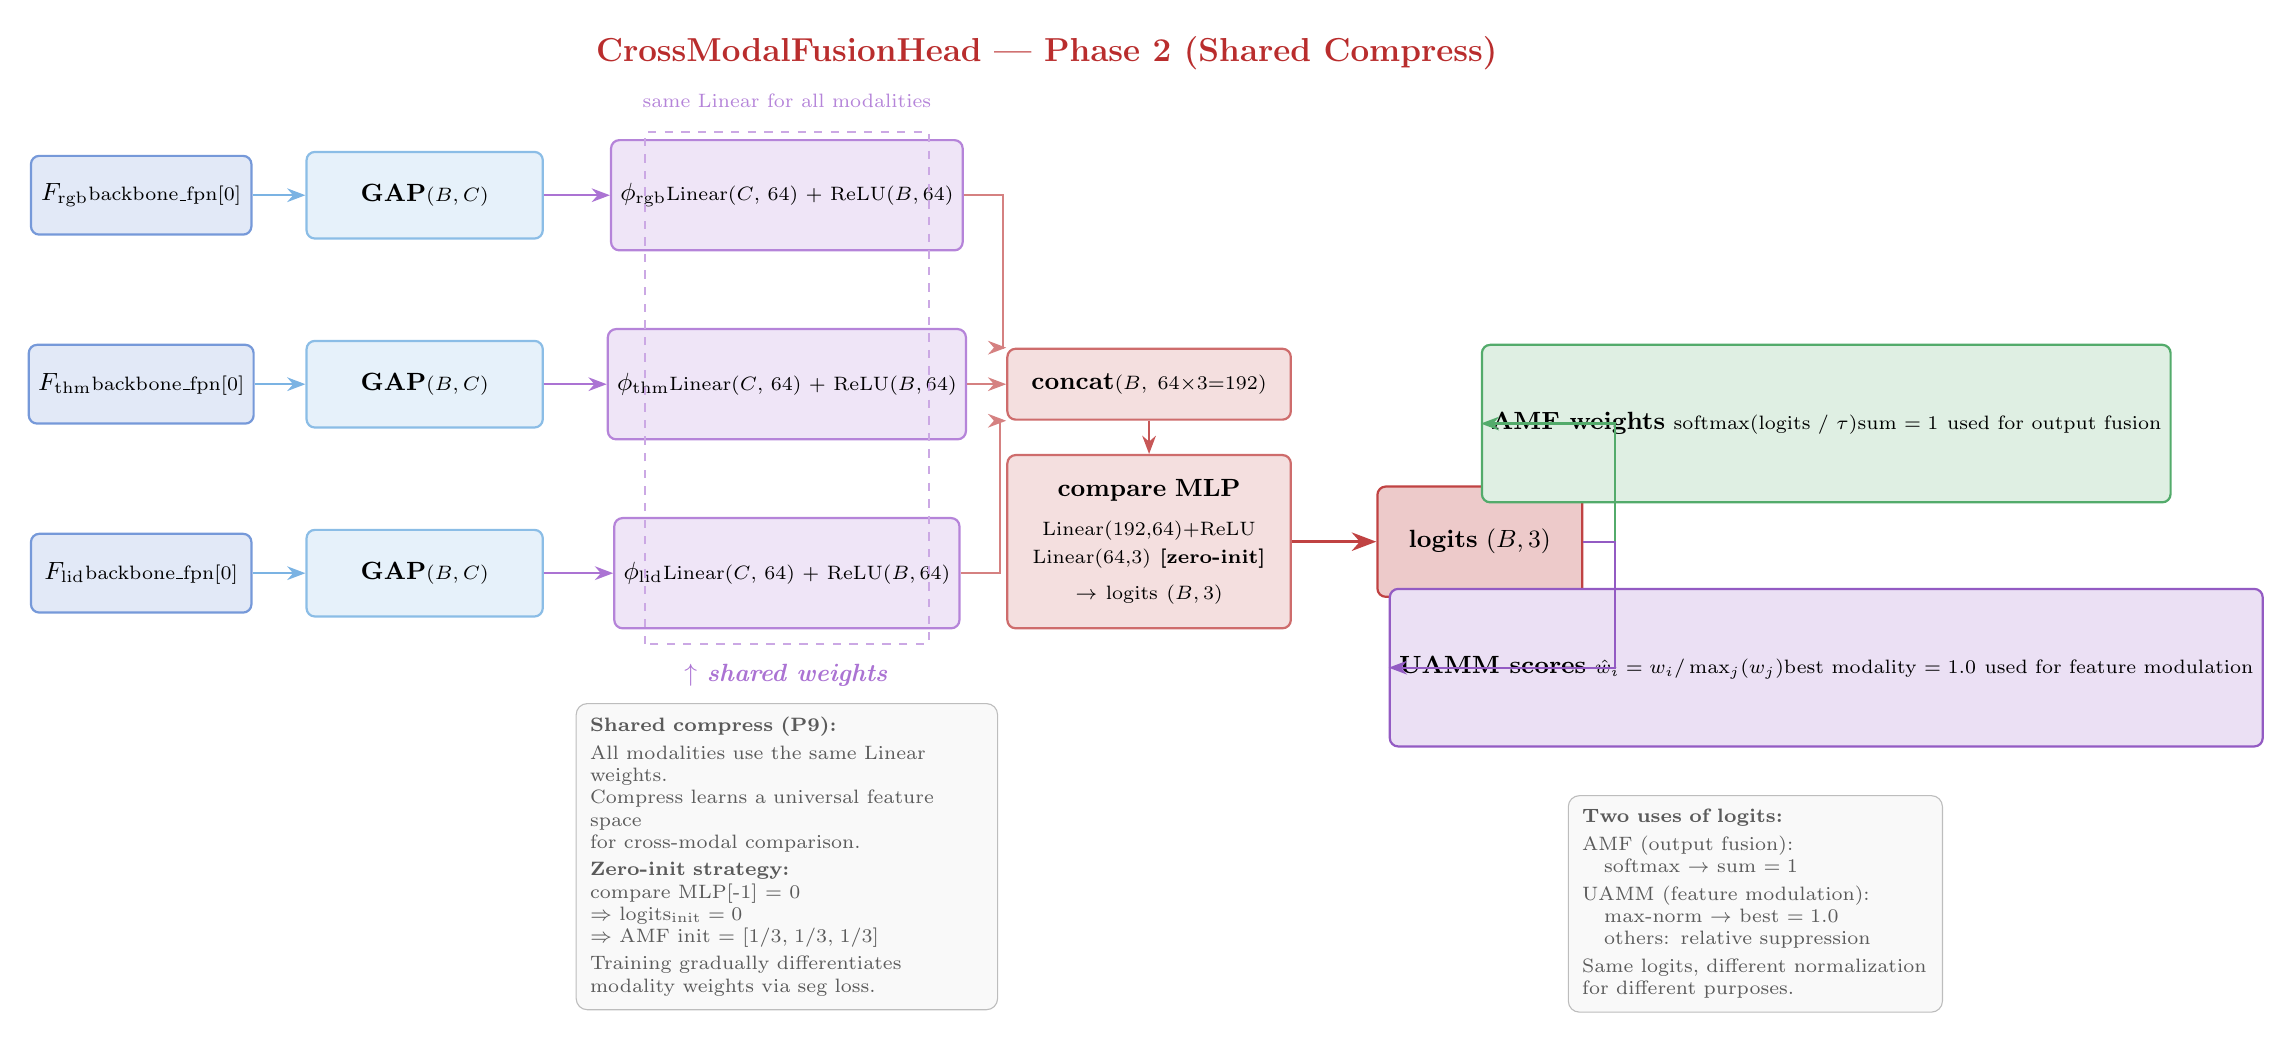
\begin{tikzpicture}

%% Layout:
%% x: 0=feat, 3.6=pool, 8.4=shared_compress, 13.0=concat, 16.4=mlp, 19.8=logits, 23.4=out
%% y: 2.4=rgb, 0.0=thm, -2.4=lid

%% ─── Title ───────────────────────────────────────────────────────
\node[font=\large\bfseries, text=cMLP] at (11.5, 4.2)
  {CrossModalFusionHead --- Phase~2 (Shared Compress)};

%% ─── backbone features ──────────────────────────────────────────
\node[feat] (fR) at (0, 2.4)  {$F_\text{rgb}$\\{\scriptsize backbone\_fpn[0]}};
\node[feat] (fT) at (0, 0.0)  {$F_\text{thm}$\\{\scriptsize backbone\_fpn[0]}};
\node[feat] (fL) at (0,-2.4)  {$F_\text{lid}$\\{\scriptsize backbone\_fpn[0]}};

%% ─── GAP (per modality, same operation) ─────────────────────────
\node[pool, minimum height=11mm] (gR) at (3.6, 2.4)
  {\textbf{GAP}\\{\scriptsize $(B,C)$}};
\node[pool, minimum height=11mm] (gT) at (3.6, 0.0)
  {\textbf{GAP}\\{\scriptsize $(B,C)$}};
\node[pool, minimum height=11mm] (gL) at (3.6,-2.4)
  {\textbf{GAP}\\{\scriptsize $(B,C)$}};

\draw[A, cPool!80] (fR)--(gR);
\draw[A, cPool!80] (fT)--(gT);
\draw[A, cPool!80] (fL)--(gL);

%% ─── Shared compress (same weights for all modalities) ───────────
\node[comp, minimum height=14mm] (cR) at (8.2, 2.4)
  {$\phi_\text{rgb}$\\{\scriptsize Linear($C$, 64) + ReLU}\\{\scriptsize $(B,64)$}};
\node[comp, minimum height=14mm] (cT) at (8.2, 0.0)
  {$\phi_\text{thm}$\\{\scriptsize Linear($C$, 64) + ReLU}\\{\scriptsize $(B,64)$}};
\node[comp, minimum height=14mm] (cL) at (8.2,-2.4)
  {$\phi_\text{lid}$\\{\scriptsize Linear($C$, 64) + ReLU}\\{\scriptsize $(B,64)$}};

\draw[A, cComp!80] (gR)--(cR);
\draw[A, cComp!80] (gT)--(cT);
\draw[A, cComp!80] (gL)--(cL);

%% Shared weights annotation
\node[font=\small\bfseries, text=cComp!80] at (8.2, -3.7)
  {$\uparrow$ \textit{shared weights}};
\draw[cComp!50, dashed, thick] (6.4,-3.3) rectangle (10.0, 3.2);
\node[font=\scriptsize, text=cComp!70] at (8.2, 3.6)
  {same Linear for all modalities};

%% ─── concat ──────────────────────────────────────────────────────
\node[mlpB, minimum height=9mm] (cat) at (12.8, 0.0)
  {\textbf{concat}\\{\scriptsize $(B,\;64{\times}3{=}192)$}};

\draw[A, cMLP!60] (cR.east)--++(5mm,0) |- (cat.north west);
\draw[A, cMLP!60] (cT.east)--(cat.west);
\draw[A, cMLP!60] (cL.east)--++(5mm,0) |- (cat.south west);

%% ─── compare MLP ─────────────────────────────────────────────────
\node[mlpB, minimum height=22mm, text width=33mm] (mlp) at (12.8,-2.0)
  {\textbf{compare MLP}\\[3pt]
   {\scriptsize Linear(192,64)+ReLU}\\[-1pt]
   {\scriptsize Linear(64,3) \textbf{[zero-init]}}\\[2pt]
   {\scriptsize $\to$ logits $(B,3)$}};

\draw[A, cMLP!80] (cat.south)--(mlp.north);

%% ─── logits ──────────────────────────────────────────────────────
\node[mlpB, minimum height=14mm, minimum width=26mm,
      fill=cMLP!25, draw=cMLP!90] (log) at (17.0, -2.0)
  {\textbf{logits} $(B,3)$};

\draw[A, cMLP!90, line width=1.3pt] (mlp.east)--(log.west);

%% ─── AMF weights ─────────────────────────────────────────────────
\node[amfB, minimum height=20mm] (amf) at (21.4, -0.5)
  {\textbf{AMF weights}\\[2pt]
   {\scriptsize softmax(logits / $\tau$)}\\
   {\scriptsize sum $= 1$}\\[2pt]
   {\scriptsize used for output fusion}};

%% ─── UAMM scores ─────────────────────────────────────────────────
\node[uamB, minimum height=20mm] (uam) at (21.4, -3.6)
  {\textbf{UAMM scores}\\[2pt]
   {\scriptsize $\hat{w}_i = w_i / \max_j(w_j)$}\\
   {\scriptsize best modality $= 1.0$}\\[2pt]
   {\scriptsize used for feature modulation}};

\draw[A, cAMF!80,  thick] (log.east)--++(4mm,0) |- (amf.west);
\draw[A, cUAMM!80, thick] (log.east)--++(4mm,0) |- (uam.west);

%% ─── annotations ─────────────────────────────────────────────────
\node[note, text width=50mm] at (8.2,-6.0) {
  \textbf{Shared compress (P9):}\\[2pt]
  All modalities use the same Linear weights.\\
  Compress learns a universal feature space\\
  for cross-modal comparison.\\[2pt]
  \textbf{Zero-init strategy:}\\
  compare MLP[-1] = 0\\
  $\Rightarrow$ logits$_\text{init} = 0$\\
  $\Rightarrow$ AMF init $=$ [1/3,\;1/3,\;1/3]\\[2pt]
  Training gradually differentiates\\
  modality weights via seg loss.
};

\node[note, text width=44mm] at (20.5,-6.6) {
  \textbf{Two uses of logits:}\\[2pt]
  AMF (output fusion):\\
  \quad softmax $\to$ sum $= 1$\\[2pt]
  UAMM (feature modulation):\\
  \quad max-norm $\to$ best $= 1.0$\\
  \quad others: relative suppression\\[2pt]
  Same logits, different normalization\\
  for different purposes.
};

\end{tikzpicture}
\end{document}
